\chapter{SPQR trees}

Before we show another interesting structure called SPQR-trees note that they are not related to the previously mentioned PQ-trees. Also in this section we will be considering multigraphs without loops, i.e. graphs can have parallel edges.

\begin{defn}
	Let $G = (V_G, E_G)$ be a biconnected multigraph, a \textbf{skeleton} of $G$ is multigraph $H = (V_H, E_H)$ with these properties:
	
	\begin{enumerate}
		\item $V_H \subseteq V_G$;
		\item every edge $e = \{u,v\} \in E_H$ represents a connected subgraph $G_e$ of $G$ ("pertinent graph of $e$") which contains the vertices $u,v$;
		\item every edge of $G$ belongs to exactly one pertinent graph;
		\item for $e,f \in E_H, e \neq f$, then $V(G_e) \cap V(G_f) = e \cap f$.
	\end{enumerate}
\end{defn}

\begin{figure}[!ht]\centering
	\begin{subfigure}{.5\textwidth}\centering
		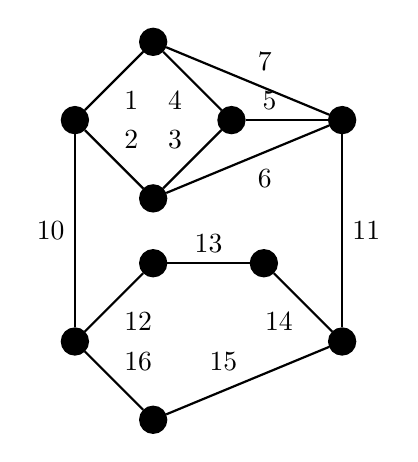
\begin{tikzpicture}[node distance = 40, main/.style = {draw, circle, fill}, thick]
			\node[main] (1) {};
			\node[main, above right of = 1] (2) {};
			\node[main, below right of = 1] (3) {};
			\node[main, above right of = 3] (4) {};
			\node[main, right of = 4] (5) {};
			\node[below of = 1] (p1) {};
			\node[main, below of = p1] (6) {};
			\node[below of = 5] (p5) {};
			\node[main, below of = p5] (7) {};
			\node[main, above right of = 6] (8) {};
			\node[main, above left of = 7] (9) {};
			\node[main, below right of = 6] (10) {};
			\draw (1) -- (2) node[midway, below right] {1};
			\draw (1) -- (3) node[midway, above right] {2};
			\draw (3) -- (4) node[midway, above left] {3};
			\draw (2) -- (4) node[midway, below left] {4};
			\draw (4) -- (5) node[midway, above left] {5};
			\draw (3) -- (5) node[midway, below right] {6};
			\draw (2) -- (5) node[midway, above right] {7};
			\draw (1) -- (6) node[midway, left] {10};
			\draw (5) -- (7) node[midway, right] {11};
			\draw (6) -- (8) node[midway, below right] {12};
			\draw (8) -- (9) node[midway, above] {13};
			\draw (7) -- (9) node[midway, below left] {14};
			\draw (7) -- (10) node[midway, above left] {15};
			\draw (6) -- (10) node[midway, above right] {16};	
		\end{tikzpicture}
		\caption{Original graph $G$.}
	\end{subfigure}
	\begin{subfigure}{.3\textwidth}
		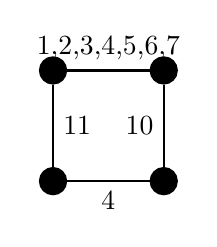
\begin{tikzpicture}[node distance = 40, main/.style = {draw, circle, fill}, thick]
			\node[main] (1) {};
			\node[main, left of = 1] (2) {};
			\node[main, below of = 1] (3) {};
			\node[main, below of = 2] (4) {};
			\draw (1) -- (2) node[midway, above] {1,2,3,4,5,6,7};
			\draw (1) -- (3) node[midway, left] {10};
			\draw (2) -- (4) node[midway, right] {11};
			\draw (3) -- (4) node[midway, below] {4};
		\end{tikzpicture}
		\caption{One skeleton.}
	\end{subfigure}
	\caption{Example of graph $G$ and some of its skeletons.}
\end{figure}

\begin{defn}
	\textbf{Separation tree $T$} of a biconnected $G = (V_G, E_G)$ is a tree whose leaves correspond bijectively to edges of $G$, every internal node $\alpha$ has degree $\geq 3$ and has an associated skeleton $S_\alpha$ of $G$ with $\deg(\alpha)$ edges, such that the edge sets of the pertinent graphs of $S_\alpha$ correspond to the sets of leaves in the components of $T - \alpha$.
\end{defn}